% \iffalse
\let\negmedspace\undefined
\let\negthickspace\undefined
\documentclass[journal,12pt,twocolumn]{IEEEtran}
\usepackage{cite}
\usepackage{amsmath,amssymb,amsfonts,amsthm}
\usepackage{algorithmic}
\usepackage{graphicx}
\usepackage{textcomp}
\usepackage{xcolor}
\usepackage{txfonts}
\usepackage{listings}
\usepackage{enumitem}
\usepackage{mathtools}
\usepackage{gensymb}
\usepackage{comment}
\usepackage[breaklinks=true]{hyperref}
\usepackage{tkz-euclide} 
\usepackage{listings}
\usepackage{gvv}                                        
\def\inputGnumericTable{}                                 
\usepackage[latin1]{inputenc}                                
\usepackage{color}                                            
\usepackage{array}                                            
\usepackage{longtable}                                       
\usepackage{calc}                                             
\usepackage{multirow}                                         
\usepackage{hhline}                                           
\usepackage{ifthen}                                           
\usepackage{lscape}
\usepackage{caption}
\newtheorem{theorem}{Theorem}[section]
\newtheorem{problem}{Problem}
\newtheorem{proposition}{Proposition}[section]
\newtheorem{lemma}{Lemma}[section]
\newtheorem{corollary}[theorem]{Corollary}
\newtheorem{example}{Example}[section]
\newtheorem{definition}[problem]{Definition}
\newcommand{\BEQA}{\begin{eqnarray}}
\newcommand{\EEQA}{\end{eqnarray}}
\newcommand{\define}{\stackrel{\triangle}{=}}
\theoremstyle{remark}
\newtheorem{rem}{Remark}
\begin{document}
\parindent 0px
\bibliographystyle{IEEEtran}
\vspace{3cm}

\title{NCERT 11.9.3 1Q}
\author{EE23BTECH11013 - Avyaaz$^{*}$% <-this % stops a space
}
\maketitle
\newpage
\bigskip

\renewcommand{\thefigure}{\arabic{figure}}
\renewcommand{\thetable}{\arabic{table}}
\large\textbf{\textsl{Question:}}
Find the $20^{th}$ and $n^{th}$ terms of the G.P $\frac{5}{2}$, $\frac{5}{4}$, $\frac{5}{8}$,.....

\solution
 \begin{table}[htbp]
     \centering
     \setlength{\extrarowheight}{8pt}
    \begin{tabular}{|c|c|c|}
    \hline
    \textbf{Parameter} & \textbf{Description} & \textbf{Value} \\
    \hline
     \(x(0)\) & First Term &\(\dfrac{5}{2}\) \\
    \hline
     \(r\) = \(\dfrac{x(1)}{x(0)}\) & Common Ratio & \(\dfrac{1}{2}\) \\
    \hline
      \(x(n)\) & \(n^{th}\) Term & \(\dfrac{5}{2}\left(\dfrac{1}{2}\right)^n \cdot u(n)\) \\
    \hline
     \(x(19)\) & \(20^{th}\) Term &\(\dfrac{5}{2} \left(\dfrac{1}{2}\right)^{19}\) \\
    \hline
     \(u(n)\) &Unit step function & \\
    \hline
  \end{tabular}

     \caption{Parameters}
     \label{tab:input__parameters1.1}
 \end{table} 

% \begin{align}
%    x(n) = \dfrac{5}{2}\left(\dfrac{1}{2}\right)^n 
% \end{align}

% \begin{align}
% 	x \brak{n} & \system{Z} X \brak{z} \\
%    % x(n) &=\dfrac{5}{2}\left(\dfrac{1}{2}\right)^n u(n) \\
%     \therefore X(z) &= \sum_{n=-\infty}^{\infty}x(n)z^{-n}\label{eq:z-transform}  
% \end{align}
% Here, 
%          $    u(n) = \begin{cases}
%                 0 &\text{for } n < 0 \\
%                 1 & \text{for } n \geq 0
%             \end{cases}$       
 
%  \vspace{1cm}
From \tabref{tab:input__parameters1.1}:
\(Z\)-Transform of \(x(n)\):
\begin{align}
% \implies X(z) &= \sum_{n=-\infty}^{\infty}\left(\dfrac{5}{2}\left(\dfrac{1}{2}\right)^n u(n)\right) z^{-n} \\
 % \implies X(z) &= \dfrac{5}{2}\sum_{n=0}^{\infty}\left(\dfrac{z
 % ^{-1}}{2}\right)^n \\
\implies X(z) &=\dfrac{5}{2}\left(\dfrac{1}{1-\frac{z^{-1}}{2}}\right) ;\cbrak{z\in\mathbb{C} : |z|>\dfrac{1}{2}}
\end{align}

\begin{figure}[ht]
    \centering
    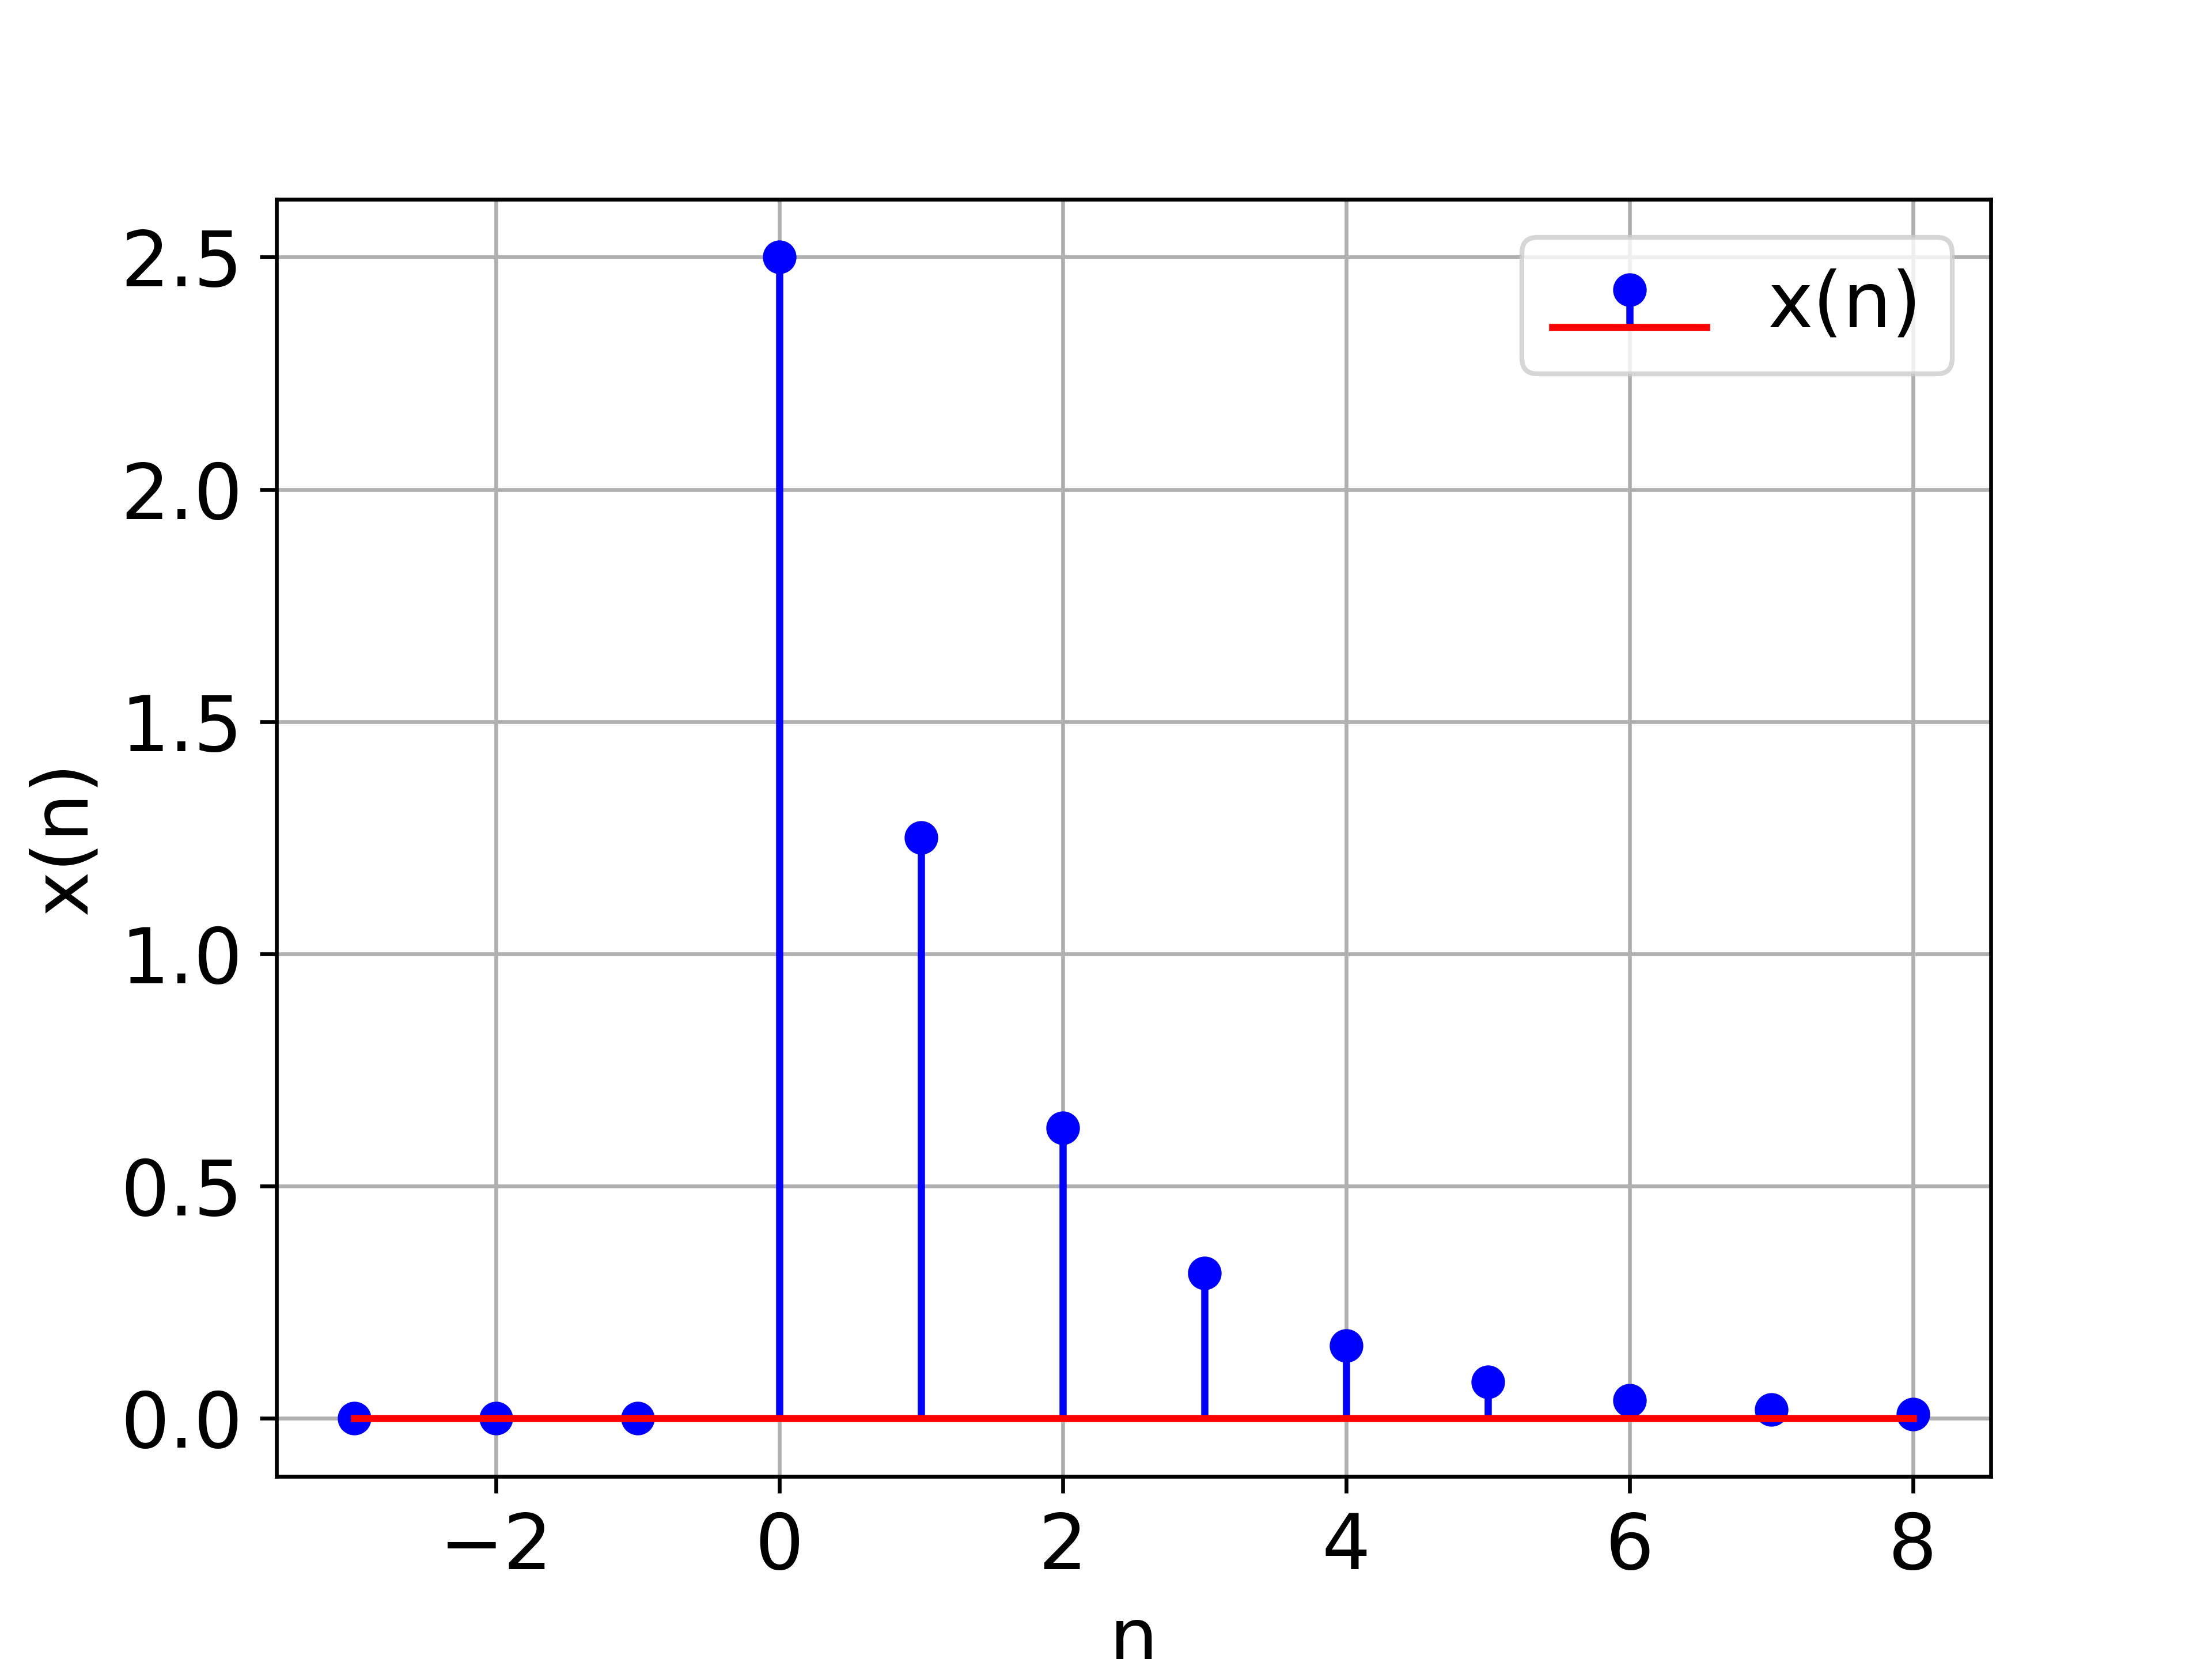
\includegraphics[width = \columnwidth]{figs/stem_plot.png}
    \caption{}
	\label{fig:x(n)_vs_n_graph1.1}
\end{figure} 

\bibliographystyle{IEEEtran}
\end{document}
